\leadchapter{
  This chapter is a general introduction to the Hawkes processes and the challenges explored in this manuscript.
  After a succinct presentation of the Hawkes processes with excitation, 
  we contextualise the state-of-the-art literature concerning estimation methods in Section~\ref{sec:chap0_introduction}. 
  This allows us to exhibit the two paradigms that are studied in this work: inhibtion and imperfect data. 
  A general outline of this manuscript is described in Section~\ref{sec:chap0_outline} along with the main questions that guided our research.
  Section~\ref{sec:chap0_inhibition} pertains to the parametric estimation of both univariate and multivariate Hawkes processes with eventual inhibiting interactions (Chapters~\ref{chapter:univariate_inhibition} and \ref{chapter:multivariate_inhibition}).
  Section~\ref{sec:chap0_missing_data} presents our contributions to the study of exciting Hawkes processes by accounting for certain models of imperfect data (Chapters~\ref{chapter:spectral_superposition} and \ref{chapter:spectral_thinning}).
}

\chapter{Introduction}

\section{Statistics for Hawkes processes: the mathematical setting}
    \subsection{At the origin: a self-exciting point process}
    %\textbf{Point processes.}
    In probability and statistics, the modelling of random collections of points in a certain space is commonly done through a point process.
    This particular version of stochastic processes is constructed around studying the spatial distribution of such indivisible elements.
    When studying point processes in the real line $\RR$ (or the half line $\RR_{\geq 0}$), the natural order of this space often incurs an ordering of any countable sequence of points $(T_k)_{k\in\ZZ}$: we talk then of \emph{temporal} point processes.

    In statistics, it is a common question to try and analyse the dynamics behind the occurrences of a certain phenomenon: the time of arrival of buses at a bus stop, the apparition of symptoms in a population or earthquake incidents in a region of the world.
    The simplest of models for point processes is the homogenenous Poisson process, where the waiting time between any two event times is distributed as an exponential random variable with a parameter $\lambda > 0$ known as the intensity of the process.
    A natural extension of this model is obtained by allowing the intensity to be a deterministic non-negative function $\lambda:\RR \to \RR_{\geq0}$, adding a temporal dependance to point arrivals.
    The more complex becomes the phenomena at the center of a study, the more intricate becomes the modelling of point processes as a result. 

    \textbf{The Hawkes process.}
    In 1971, Alan G. Hawkes introduced his model of self-exciting point processes \parencite{Hawkes1971}, which would come to be known later as the Hawkes point process.
    He defines this model through a past-dependant intensity function $\lambda:\RR\to\RR_{>0}$, that for any instant in time $t$, the intensity is expressed through the history $\mathcal{H}_t$ of process $N$ up to $t$, and was originally defined as:
    \begin{equation}\label{eq:chap0_univariate_linear_intensity}
        \lambda(t\mid \mathcal{H}_t) = \mu + \sum_{T_k \leq t}{h(t-T_k)}\,.
    \end{equation}

    The term $\mu$ is often referred to as the baseline intensity, which similar to the homogeneous Poisson process, dictates a constant rate of occurrences. 
    The dependance on the past is represented by the second term, where each event time that precedes $t$ contributes to the intensity function through the interaction function $h:\RR_{\geq0}\to\RR_{>0}$.

    It is mainly through this interaction function, also called kernel function, that the effects of the past are modelled. 
    The positivity of $h$ represents an excitation effect between points: each time an event $T_k$ occurs, it increases the value of the intensity function, increasing in turn the rate at which points appear.
    For stability reasons, $h$ is assumed to converge to $0$ as $t\to+\infty$, representing the dissipation of effects as time advances.

    Different shapes of $h$ allow to account for different effects. 
    On the one hand, strictly decreasing functions represent instantaneous effects such as the exponential or power-law kernels, which appear as spikes in the conditional intensity function. 
    On the other hand, the Rayleigh or gamma kernels can be chosen to represent delayed effects, where the maximum of the function is not at the origin $t=0$. Figure~\ref{fig:chap0_two_kernel_examples} illustrates two Hawkes processes with two different kernels.
    The properties of the conditional intensity function are intrinsically connected to those of $h$, and so when working in parametric settings, the choice of the kernel is essential and come with their advantages and inconveniences.
    The choice of smooth functions is transcribed as smoothness between two consecutive event times whereas the choice of kernels with bounded supports allow to leverage results from renewal process theory.

    \begin{figure}[!ht]
        \centering
          \includegraphics[width=\textwidth]{images/chapter0/two_kernel_examples.pdf}
        \caption{Kernel functions (top) and respective conditional intensity (bottom) functions of a Hawkes process started at $t=0$ for exponential (left) and gamma (right) parametrisations.
        }
        \label{fig:chap0_two_kernel_examples}
      \end{figure}

    \textbf{Clustering and branching structures.}
    A direct consequence of the expression of the intensity function as in Equation~\eqref{eq:chap0_univariate_linear_intensity} is that the Hawkes process model can be interpreted as a Poisson cluster process \parencite{Hawkes1974}.
    The most practical way of defining a cluster point process is as from a generative point of view.
    We begin by generating a homogenenous Poisson process in the real line $\RR$ with parameter $\mu$: these points $T_k^c$ are often called ancestors, immigrants or cluster centers.
    Each center generates a inhomogeneous Poisson process with intensity function $h(\cdot - T_k^c)$, forming a family of children points, also called descendants.
    The iteration is repeated with each new point generating its own subprocess until no descendants are generated.
    In the end, the cluster process, which with these notations would be a Hawkes process, is formed by the union of both ancestors and descendants.
    What distinguishes a Hawkes process is the fact that the support of the function $h$ is a subset of $\RR_{\geq0}$, meaning that each occurrence influences solely the future of the process.

    % Add a table with common kernels

    Aside from being a cluster Poisson process, we may remark that the generation algorithm describes a dynamic similar to a Galton-Watson branching process (see \textcite{Watson1875} for the discrete time version and \textcite[Chapter III]{Harris02} for the generalised version).
    More precisely, the Hawkes process can be seen as a time-continuous branching process with immigration:
    let us assume we observe the arrival of an immigrant at a time $T_k^c$.
    This immigrant will generate a first generation of children forming the first generation of points, or branches.
    As before, each child becomes its own parent by generating a new set of branches.
    A tree is then formed by the union of each immigrant and all of its descendants, and then the Hawkes process is once again formed by the union of all trees.

    A visualisation of both structures is illustrated in Figure~\ref{fig:branching_and_cluster05} for a Hawkes process with exponential kernel. 
    These two properties are what made Hawkes processes so attractive in the literature.
    From a theoretical point of view, the many existing developments of branching theory allowed to quickly obtain results concerning existence, stability, stationarity and other descriptors of the process.
    A main example concerns the existence of a Hawkes process: in order for the point process to have a finite number of points inside any bounded set, a necessary and sufficient condition is:
    \[\int_{0}^{+\infty}{h(t)\dd t} < 1\,.\]
    From a numerical point of view, we already introduced a simulation algorithm as described by the cluster structure and methods of estimation from both fields could be adapted in order to study Hawkes processes.
    
    \begin{figure}[!ht]
        \centering
          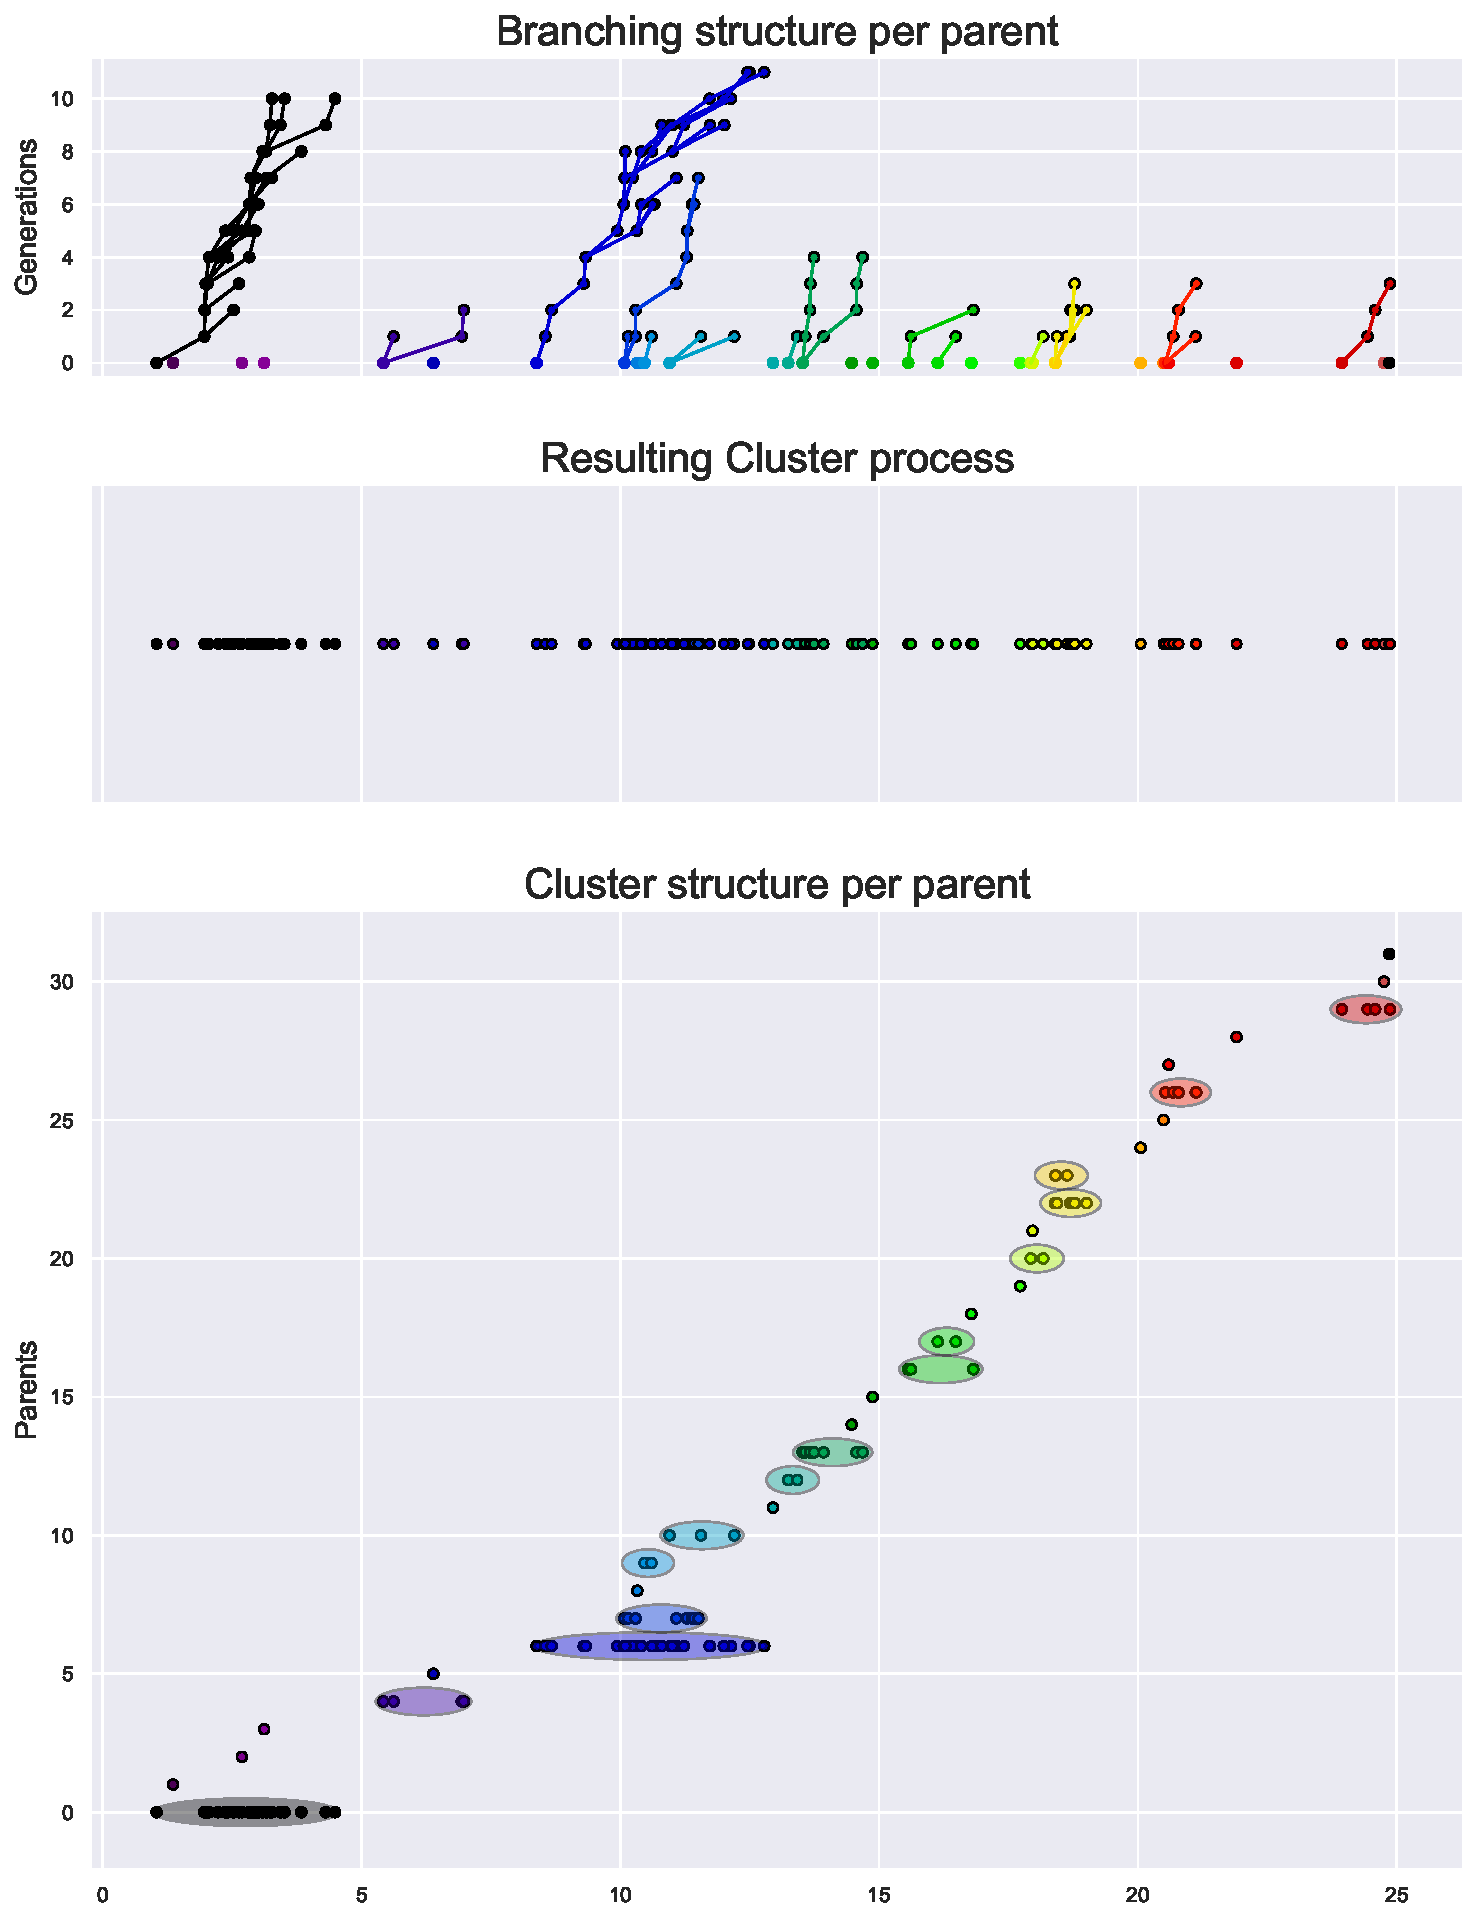
\includegraphics[width=0.95\textwidth]{images/chapter0/branching_and_cluster05.pdf}
        \caption{Illustration of both branching (top) and clustering (bottom) structures of an exponential Hawkes process (middle). Each color represents a single cluster/tree. Simulation is done through the cluster process algorithm.
        }
        \label{fig:branching_and_cluster05}
      \end{figure}

    It is these properties, and the quick developments that followed in the literature, that created a growing interest in other scientific fields.
    From this, different versions of the original self-exciting Hawkes process appeared in the literature, each one trying to accomodate more complex phenomena.

    \textbf{The multivariate Hawkes process.} Probably the most natural and useful was the definition of a \emph{multivariate} Hawkes process. 
    Instead of studying a single phenomenon (an univariate process), we define a $d$-variate Hawkes process as $d$ individual point processes $(N_i)_{i=1:d}$, 
    where each process is defined by a conditional intensity function $\lambda^i$:
    \[\lambda^i(t) = \mu_i + \sum_{j=1}^{d}\sum_{T_k^j \leq t}{h_{ij}(t-T_k^j)}\,, \qquad \text{for any $t\in\RR$.}\]

    In this formulation, each process $N^j$ has its own event times $(T_k^j)_{k\in\ZZ}$ and baseline intensity $\mu_i > 0$.
    What makes this model so interesting is the fact that it introduces interaction between processes, which is seen in the second term of the intensity.
    The kernel functions $h_{ij}$ represent the effect of points from $N^j$ on process $N^i$.
    This model allows to study a group of individuals linked by a network of interactions, adding a new dimension of study for such processes.

    From modelling infection spread all the way to the study of clusters of earthquakes, approaching the study of Hawkes processes from a statistical point of view quickly became a necessity.

    \subsection{Inference and applications}

    \textbf{Statistical estimation.}
    Presenting an exhausting bibliography on statistical estimation for Hawkes processes would represent a titanical task, 
    specially due to the numerous alternative models introduced since their introduction.
    Nonetheless, we propose here a general overview of the estimation panorama in the literature for self-exciting Hawkes processes.
    
    Statistical models for Hawkes processes with excitation focus around estimating both the baseline intenisty $\mu$ and the interation function $h$.
    In parametric settings, many kernel functions are traditionnally used (as some mentioned in the previous section),
    each one defined by a parameter $\gamma\in\RR^m$ for a certain integer $m$.

    %\Add theta and statistical model

    To our knowledge, the very first paper implementing an estimation procedure in a parametric framework is \textcite{Adamopoulos1976}.
    In his work, the author proposes a study of exponential kernels for both univariate and bivariate Hawkes processes through the spectral log-likelihood,
    closely related to time series theory.
    Let us take the time to remark that the exponential kernel is often chosen as a parametric interaction function because the univariate Hawkes process becomes a Markov process.
    This allows for many simplification when computing many quantities proper to the study of point process.
    as seen in the implementation of the maximum likelihood estimator (MLE) in \textcite{Ozaki1979}.
    The expression of the log-likelihood of a general point process, for an observation in $[0, T]$, is:
    \[\ell_T(\theta) = - \int_{0}^{T}{\lambda(u)\dd u} + \sum_{k=1}^{N(T)}{\log(\lambda(T_k))}\,,\]
    where $N(T)$ is the number of points in the observation window. 
    Other implementations of the MLE include \textcite{Ogata1988, Guo2018} and \textcite{Lewis2011} with a penalised version optimised by an EM algorithm.
    An alternative approach leveraging the branching structure is proposed in \textcite{Veen2008}.
    Other traditional methods in settings include least-squares minimisation \parencite{Reynaud2010, Eichler2016, Kirchner2017}, 
    method of moments \parencite{DaFonseca2013},
    via the solutions of Wiener-Hopf equation \parencite{Bacry2016},
    through approximation with autoregressive models \parencite{Kirchner2017},
    to name a few.
    
    All of these references concern frequentist approaches of statistics, 
    and so it is essential to mention that an equal effort has been made from a Bayesian point of view.
    \textcite{Rasmussen2013} proposes two procedures through log-likelihood estimation: 
    one through the classical intensity function and another similar to \textcite{Veen2008} with the branching structure.
    In \textcite{Lemonnier2014}, the authors propose an approximation through exponential kernels and taking advantage of the markovian properties.
    The multivariate case is deeply study in \textcite{Donnet2020} with illustrations on estimating the underlying interaction graph.
    
    This is a small insight on the plethora of approaches that have been developed in order to study these kind of processes.
    
    \textbf{Application fields.}
    The main motivation behind the works presented in this thesis, as it has been and continues to be for researches in this field,
    is to use the versatility of the model and its exceptional adaptability to propose new submodels.
    When confronted to real-world data, 
    researchers tend to reformulate and complexify the Hawkes model in order to better describe the studied phenomena. 
    
    The historical example is in seismology, 
    where the clustering structure becomes a way to study earthquakes and their replicas, as shown in \textcite{Adamopoulos1976,Ogata1988, Ogata1998} and more recent works \parencite{Kwon2023}.
    In this, the authors tend to add a spatial component to the model in order to account for both temporal and spatial dependence among points.
    %Further develop
    Including additional information in the model is a common approach, done often with marked version of the Hawkes process,
    which allows to incorporate addional covariates to the estimations. 
    In the study of social network interactions, as done in \textcite{Mishra2016,Rizoiu2017},
    by including information about each studied individual like number of followers or quality of the publications the authors improve the estimation of tweet cascades.

    Another approach is to render the baseline intensity a function of time, 
    as done in criminology \textcite{Lewis2011, Olinde2020}, 
    in order to account for changing behaviours throughout different moment of the day.

    Working in high dimensions allows to account for high number of individuals with sparse networks of interactions.
    Penalisation methods in the study of neuronal spike trains \parencite{Reynaud2013, Lambert2018}
    improve computational times and provide more explicative models of neuronal connectivity.

    Many other fields include finance \parencite{Embrechts2011, Bacry2013, Lotz2024}, TV browsing analysis \parencite{Xu2016}, event data streams in football \parencite{Baouan2023, Narayanan2023}, 
    each one often accompanied with a new formulation of the Hawkes process.

    \subsection{Outline and challenges of this manuscript.}\label{sec:chap0_outline}

    Our goal in this thesis is to study two separate extensions of the Hawkes process model: the inhibition effect and the study of imperfect data.
    As a consequence, this manuscript is divided in two parts, with Chapter~\ref{chapter:background} presenting a succinct presentation of point processes theory, from a random measure approach, and the formalism of Hawkes processes.
    Let us note that all chapters are independent of each other and can be read as standalone documents.

    The first part of this thesis (Section~\ref{sec:chap0_inhibition}) concerns the study of the inhibition: 
    the opposite effect to excitation.

    \begin{itemize}
      \item Chapter~\ref{chapter:univariate_inhibition} presents a parametric estimation method for univariate Hawkes processes that accounts for both self-exciting or self-inhibiting interactions. 
      This is a joint work with Anna Bonnet and Maxime Sangnier. 

      The corresponding paper \parencite{bonnet2021} has been published in \textit{Statistics and Probability Letters}.
      
      Code is freely available at \url{https://github.com/migmtz/hawkes-inhibition-expon}

      \item Chapter~\ref{chapter:multivariate_inhibition} presents a parametric estimation method for multivariate exponential Hawkes processes with exciting and inhibiting interactions along with a model selection procedure. 
      This is a joint work with Anna Bonnet and Maxime Sangnier. 

      The corresponding paper \parencite{Bonnet2023} has been published in \textit{Statistics and Computing}.
      
      Code is freely available at \url{https://github.com/migmtz/multivariate-hawkes-inhibition}

    \end{itemize}

    The second part (Section~\ref{sec:chap0_missing_data}) consists in the study of imperfect observations of a Hawkes process realisation, similar to missing data formulations.

    \begin{itemize}
      \item Chapter~\ref{chapter:spectral_superposition} presents a parametric estimation method for exciting Hawkes processes whose event times are noised by those of a homogenenous point process, leveraging point process spectral theory. 
      This is a joint work with Anna Bonnet, Felix Cheysson and Maxime Sangnier. 

      The corresponding paper \parencite{Bonnet2024} has been submitted for publication.

      Code is available at \url{https://github.com/migmtz/noisy-hawkes-process}

      \item Chapter~\ref{chapter:spectral_thinning} presents the analysis of an inference method for thinned univariate Hawkes processes through spectral theory. 
      Additionally, it presents an improvement of $\ell_2$ penalisation through thinning subsampling for the spectral estimator.

      This chapter is an ongoing joint work with Felix Cheysson.
    \end{itemize}
    


    %\subsection{Questions} %and contributions}
    \begin{itemize}
        %\item In this thesis we study two extensions: 
        %\item In the first half (chapters) we study inhibition 
        %\item In the second half (chapters) we study missing data.
        \item Our studies are articulated along 3 general questions (i) what approaches for considering alternative or more complex dynamics than self-excitation in parametric and what properties can we establish; (ii) how to evaluate and select our models through data-based methods in multivariate cases (null interactions); (iii) what statistical tools allow us to improve inference.
    \end{itemize}

% mentionner faire des outils accessible, partage du code (open source, facilité)
% mettre/valoriser les codes ici 
\section{Encouraging restraint: factoring in inhibition for Hawkes processes}\label{sec:chap0_inhibition}
    \begin{itemize}
        \item Introduce the non-linear HP and give reference to other models of inhibition 
        \item Define inhibition in our case
        \item Bibliography of pre-existing methods (non parametric, bayesian).
    \end{itemize}
    \subsection{Maximum Likelihood Estimation for Hawkes Processes with self-excitation or inhibition}
    Summary

    \subsection{Inference of multivariate exponential Hawkes processes with inhibition and application to neuronal activity}
    Extension of previous chapter to multivariate
    Real data application and methods for better.

    % By allowing the interaction function $h$ to take negative values,
    % the occurrence of a point \emph{decreases} the rate of incoming event times.
    % The main difficulty of this approach originates from the non-negativity requirement on the conditional intensity function.
    % This is often controlled by introducing the concept of \emph{non-linear} Hawkes processes.

\section{Something is amiss: spectral methods for missing data}\label{sec:chap0_missing_data}
    \begin{itemize}
        \item Introduce the point process operations and provide missing data formalism. 
        \item Bibliography
    \end{itemize}
    \subsection{Spectral analysis for the inference of noisy Hawkes processes}
    Summary
    
    \subsection{A numerical exploration of thinned Hawkes processes through spectral theory}
    Inspired by previous but also better methods.


%entrer titre et outline